\section{Resultados} \label{sec:resultado}

\subsection{Blur (\texttt{h2} e \texttt{h6})} \label{sec:blur}

    Os filtros mais simples de identificar foram os de \textit{blur}, que fazem um tipo de média ponderada da vizinhaça do pixel.

\begin{figure}[H]
    \centering
    \begin{subfigure}{0.4\textwidth}
        \centering
        \begin{kmatrix}
    \matrix(img)[square matrix]{
        1 & 4 & 6 & 4 & 1 \\
        4 & 6 & 24 & 6 & 4 \\
        6 & 24 & 36 & 24 & 6 \\
        4 & 6 & 24 & 6 & 4 \\
        1 & 4 & 6 & 4 & 1 \\
    };

    \node[left=of img] {$\displaystyle\Scale[1.7]{\frac{1}{256}}$};
\end{kmatrix}
        \caption{~$h_2$}
        \label{fig:h2}
    \end{subfigure}%
    \begin{subfigure}{0.4\textwidth}
        \centering
        \begin{kmatrix}
    \matrix(img)[square matrix]{
        1 & 1 & 1 \\
        1 & 1 & 1 \\
        1 & 1 & 1 \\
    };

    \node[left=of img] {$\displaystyle\Scale[1.7]{\frac{1}{9}}$};
\end{kmatrix}
        \caption{~$h_6$}
        \label{fig:h6}
    \end{subfigure}

    \caption{Máscaras de \textit{blur}.}
    \label{fig:blur:kernel}
\end{figure}

O primeiro deles é o filtro gaussiano $5 \times 5$ \autocite{ref:gaussian}, que pode ser visto na \cref{fig:h2}. Essa matriz é ponderada de acordo com as distâncias 4 do pixel central, reduzindo o peso para pixels mais distantes. No espaço das frequências, esse filtro funciona como um passa-baixas, reduzindo a influência de frequências muito altas, o que pode servir para melhorar o resultado de outros filtros, como o laplaciano, ou para evitar problemas de \textit{aliasing} \autocite{ref:gaussian-lowpass}. Na \cref{fig:blur:gauss}, podemos ver o resultado de aplicar esse filtro na imagem \texttt{house.png} (\ref{fig:blur:orig}).

\begin{figure}[H]
    \centering
    \begin{subfigure}{0.48\textwidth}
        \centering
        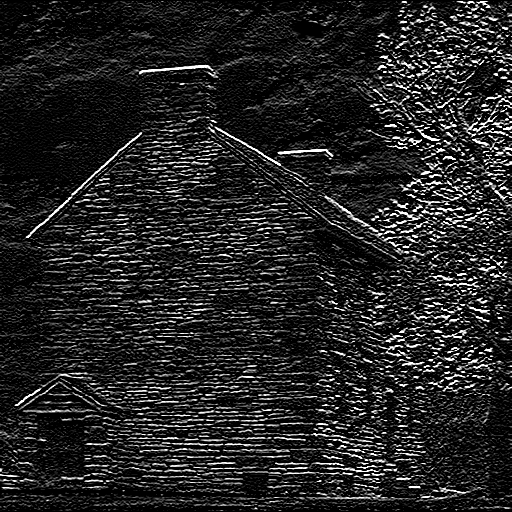
\includegraphics[width=0.9\textwidth]{imagens/house.png}
        \caption{Original: \texttt{house.png}.}
        \label{fig:blur:orig}
    \end{subfigure}\\[8pt]
    \begin{subfigure}{0.48\textwidth}
        \centering
        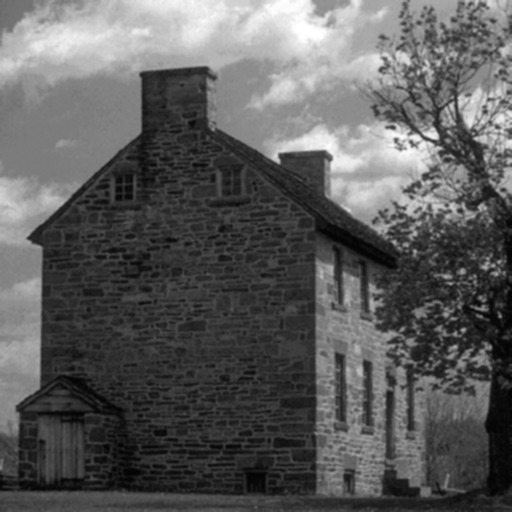
\includegraphics[width=0.9\textwidth]{resultados/house_h2.png}
        \caption{Convolução com $h_2$ (\ref{fig:h2}).}
        \label{fig:blur:gauss}
    \end{subfigure}%
    \begin{subfigure}{0.48\textwidth}
        \centering
        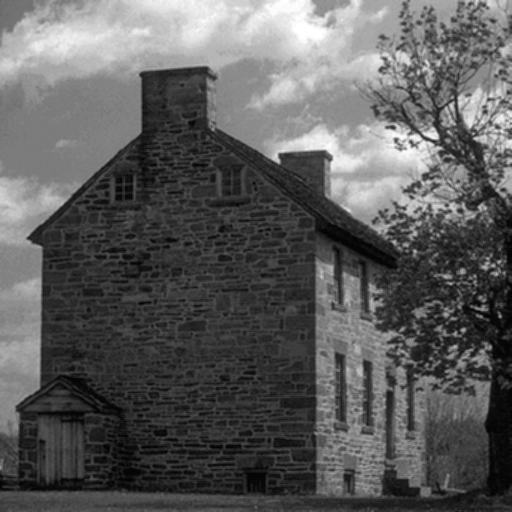
\includegraphics[width=0.9\textwidth]{resultados/house_h6.png}
        \caption{Convolução com $h_6$ (\ref{fig:h6}).}
        \label{fig:blur:box}
    \end{subfigure}

    \caption{Aplicação do \textit{blur}.}
    \label{fig:blur}
\end{figure}

O segundo filtro é chamada de \textit{box blur}, que faz uma média simples da vizinhaça 8 do pixel. Isso pode ser visto no \textit{kernel} do filtro (\cref{fig:h6}). Apesar de ser diferente do gaussiano, o resultado ficou bem parecido, como pode ser visto na \cref{fig:blur}. O motivo disso é que os pesos mais externos do filtro gaussiano $5 \times 5$ são bem baixos, fazendo com a região $3 \times 3$ seja mais presente, sendo essa a mesma região do filtro \textit{box}.

No programa, esses filtros podem ser aplicados com: \enlargethispage{20pt}

\begin{minted}{bash}
    $ python3 main.py imagens/house.png h2 # ou h6
\end{minted}


\subsection{Motion Blur (\texttt{h9})} \label{sec:motion}

    % http://users.ece.northwestern.edu/~sda690/MfB/Motion_CVPR08.pdf
% https://www.geeksforgeeks.org/opencv-motion-blur-in-python/
% https://www.wikiwand.com/en/Motion_blur
% http://tech.abdulfatir.com/2014/05/kernel-image-processing.html

Além dos filtros de \textit{blur} apresentados na \hyperref[sec:blur]{seção anterior}, temos também um filtro de \textit{blur} direcionado, muitas vezes usado para alcançar um efeito de \textit{motion blur}. Para o \textit{kernel} da \cref{fig:h9}, o \textit{blur} está direcionado a 45\textdegree, como se a câmera estivesse se movendo da esquerda-superior para a direita-inferior.

\begin{figure}[H]
    \centering
    \begin{kmatrix}
    \matrix(img)[square matrix]{
        1 & 0 & 0 & 0 & 0 & 0 & 0 & 0 & 0 \\
        0 & 1 & 0 & 0 & 0 & 0 & 0 & 0 & 0 \\
        0 & 0 & 1 & 0 & 0 & 0 & 0 & 0 & 0 \\
        0 & 0 & 0 & 1 & 0 & 0 & 0 & 0 & 0 \\
        0 & 0 & 0 & 0 & 1 & 0 & 0 & 0 & 0 \\
        0 & 0 & 0 & 0 & 0 & 1 & 0 & 0 & 0 \\
        0 & 0 & 0 & 0 & 0 & 0 & 1 & 0 & 0 \\
        0 & 0 & 0 & 0 & 0 & 0 & 0 & 1 & 0 \\
        0 & 0 & 0 & 0 & 0 & 0 & 0 & 0 & 1 \\
    };

    \node[left=of img] {$\displaystyle\Scale[1.7]{\frac{1}{9}}$};
\end{kmatrix}

    \caption{Máscara de \textit{motion blur}: $h_9$.}
    \label{fig:h9}
\end{figure}

\begin{figure}[H]
    \centering
    \begin{subfigure}{0.48\textwidth}
        \centering
        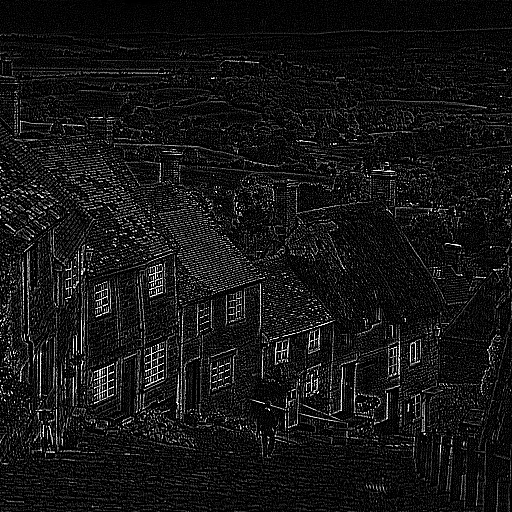
\includegraphics[width=0.9\textwidth]{imagens/city.png}
        \caption{Original: \texttt{city.png}.}
    \end{subfigure}%
    \begin{subfigure}{0.48\textwidth}
        \centering
        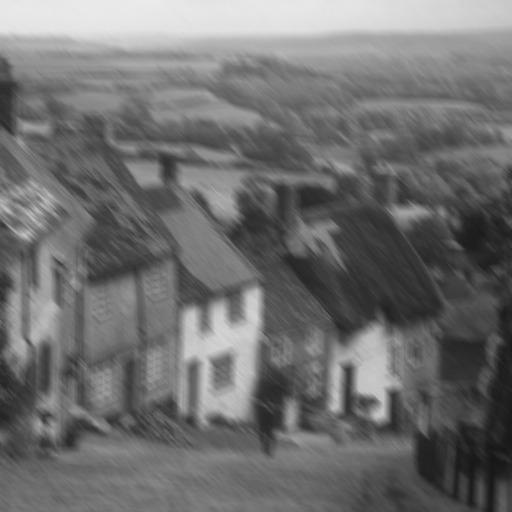
\includegraphics[width=0.9\textwidth]{resultados/city_h9.png}
        \caption{Convolução com $h_9$ (\ref{fig:h9}).}
        \label{fig:motion:conv}
    \end{subfigure}

    \caption{Aplicação de \textit{motion blur}.}
    \label{fig:motion}
\end{figure}

Para a execução pelo programa, o comando deve ser no formato abaixo, resultando em algo como a \cref{fig:motion:conv}.

\begin{minted}{bash}
    $ python3 main.py imagens/city.png h9
\end{minted}



\subsection{Detecção de Borda (\texttt{h1} e \texttt{h5})} \label{sec:borda}

    \begin{figure}[H]
    \centering
    \begin{subfigure}{0.48\textwidth}
        \centering
        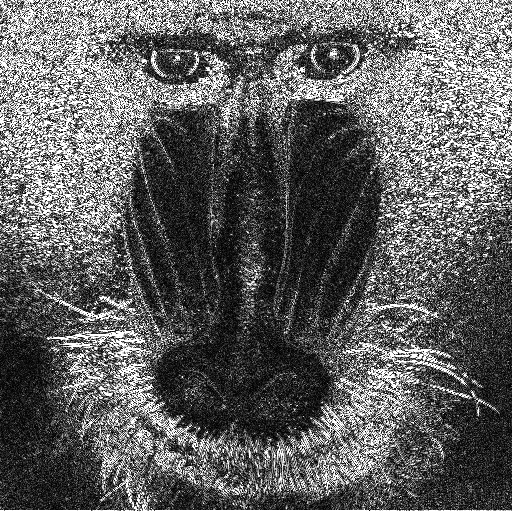
\includegraphics[width=0.9\textwidth]{imagens/baboon.png}
        \caption{Original: \texttt{baboon.png}.}
    \end{subfigure}\\[8pt]
    \begin{subfigure}{0.48\textwidth}
        \centering
        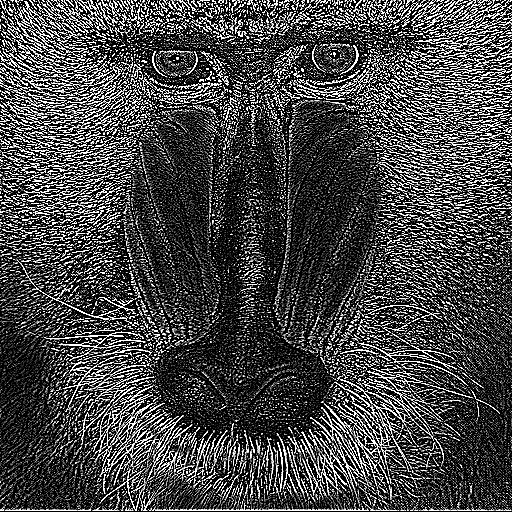
\includegraphics[width=0.9\textwidth]{resultados/baboon_h1.png}
        \caption{Convolução com $h_1$ (\ref{fig:h1}).}
        \label{fig:borda:viz4}
    \end{subfigure}%
    \begin{subfigure}{0.48\textwidth}
        \centering
        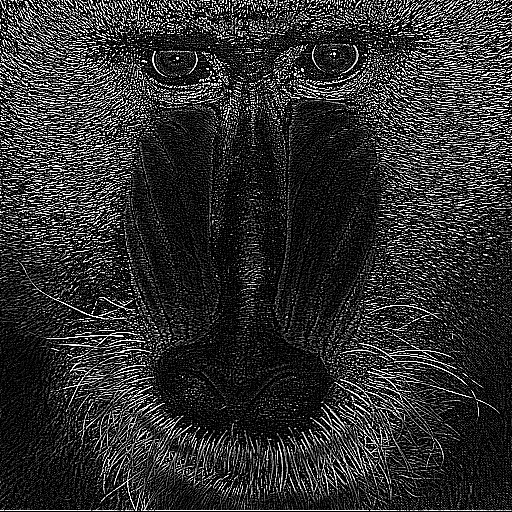
\includegraphics[width=0.9\textwidth]{resultados/baboon_h5.png}
        \caption{Convolução com $h_5$ (\ref{fig:h5}).}
        \label{fig:borda:viz8}
    \end{subfigure}

    \caption{Aplicação do laplaciano discreto.}
\end{figure}

Os filtros de detecção ou realce de bordas mais comuns são os chamados não-direcionais. Normalmente, eles são desenvolvidos a partir do operador laplaciano discreto \autocite{ref:laplacian}. Uma característica importante dos filtros de detecção de bordas é que seus elementos somam zero.

O operador laplaciano serve como uma medida de quanto uma função espacial no ponto $p$ é diferente da média dos pontos em um raio $[p - \delta r, p + \delta r]$. No caso discreto bidimensional, como imagens, existem duas principais medidas de distância, considerando as vizinhaças 4 e 8. Elas resultam em dois tipos de laplacianos diferentes, como pode ser visto na \cref{fig:borda:kernel}.

Nesse trabalho temos o \textit{kernel} $h_1$ (\ref{fig:h1}), com vizinhaça 4 de raio 2, e o $h_5$, com vizinhaça 8 de raio 1. Os resultados podem ser vistos nas figuras \ref{fig:borda:viz4} e \ref{fig:borda:viz8}, respectivamente. Podemos ver que as bordas nas regiões de baixa frequência são bem detectadas, como no centro da imagem, mas regiões de alta frequência resultam em muita informação e podem acabar atrapalhando a análise das bordas. Uma forma de contornar esse problema é aplicando um filtro passa-baixas, como o \textit{blur} gaussiano, discutido na \cref{sec:blur}.

\begin{figure}[H]
    \centering
    \begin{subfigure}{0.4\textwidth}
        \centering
        \begin{kmatrix}
    \matrix[square matrix]{
        0 & 0 & -1 & 0 & 0 \\
        0 & -1 & -2 & -1 & 0 \\
        -1 & -2 & 16 & -2 & -1 \\
        0 & -1 & -2 & -1 & 0 \\
        0 & 0 & -1 & 0 & 0 \\
    };
\end{kmatrix}
        \caption{~$h_1$}
        \label{fig:h1}
    \end{subfigure}%
    \begin{subfigure}{0.4\textwidth}
        \centering
        \begin{kmatrix}
    \matrix[square matrix]{
        -1 & -1 & -1 \\
        -1 & 8 & -1 \\
        -1 & -1 & -1 \\
    };
\end{kmatrix}
        \caption{~$h_5$}
        \label{fig:h5}
    \end{subfigure}

    \caption{Filtros laplacianos discretos}
    \label{fig:borda:kernel}
\end{figure}

A execução pode ser feita com:

\begin{minted}{bash}
    $ python3 main.py imagens/baboon.png h1
    # ou
    $ python3 main.py imagens/baboon.png h5
\end{minted}


\subsection{Operador de Sobel (\texttt{h3} e \texttt{h4})} \label{sec:sobel}

    Além dos detectores de borda não-direcionais, existem detectores que se importam com qual direção está sendo feita a análise. Muitos desses operadores são baseados na noção de gradiente, que representa matematicamente exatamente essa ideia.

Dentre eles, existe o operador de Sobel \autocite{ref:sobel}, que faz o gradiente nas direções $x$ e $y$ do plano cartesiano. Em específico, considerando a operação de convolução, o filtro $h_3$ (\ref{fig:h3}) aponta na direção $-x$ (para a esquerda) e o $h_4$ (\ref{fig:h4}), na $-y$ (para cima).

\begin{figure}[H]
    \centering
    \begin{subfigure}{0.4\textwidth}
        \centering
        \begin{kmatrix}
    \matrix[square matrix]{
        -1 & 0 & 1 \\
        -2 & 0 & 2 \\
        -1 & 0 & 1 \\
    };
\end{kmatrix}
        \caption{~$h_3$}
        \label{fig:h3}
    \end{subfigure}%
    \begin{subfigure}{0.4\textwidth}
        \centering
        \begin{kmatrix}
    \matrix[square matrix]{
        -1 & -2 & -1 \\
        0 & 0 & 0 \\
        1 & 2 & 1 \\
    };
\end{kmatrix}
        \caption{~$h_4$}
        \label{fig:h4}
    \end{subfigure}

    \caption{Máscaras de Sobel.}
    \label{fig:sobel:kernel}
\end{figure}

Observando os resultados na \cref{fig:sobel}, podemos ver que quase não existe separação do corpo da borboleta com as asas na \cref{fig:sobel:y}, isso porque ela quase não apresenta variações verticais nessa região. Nessa mesma figura, no entanto, podemos ver claramente a separação do topo da asa, que não acontece na \cref{fig:sobel:x}, já que é uma região com pouca variaçao horizontal.

Além disso, podemos ver a presença do direcinamento $-x$ em vez do $+x$ na \ref{fig:sobel:x}. Em especial, na parte inferior da asa esquerda, logo abaixo do abdômen do inseto, é bem visível a borda do componente, o que não acontece na mesma região da asa direita. No tórax da borboleta também fica visível uma separação bilateral, que não é aparente na imagem original (\ref{fig:sobel:orig}).

Muitas vezes, os operadores de Sobel são combinados para extrair informações importantes do gradiente. O mais comum, é o módulo da gradiente, que no caso é encontrado por $\sqrt{\left(h_3\right)^2 + \left(h_4\right)^2}$. Ele serve como um bom detector de borda, medindo o quão forte é a variação em cada região da imagem. O resultado pode ser visto na \cref{fig:sobel:abs}.

\begin{figure}[H]
    \centering
    \begin{subfigure}{0.48\textwidth}
        \centering
        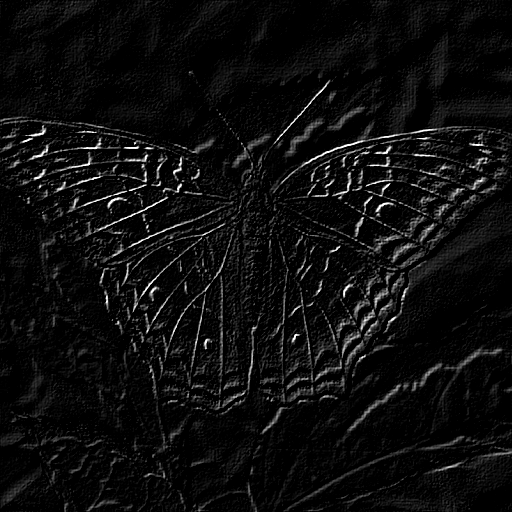
\includegraphics[width=0.9\textwidth]{imagens/butterfly.png}
        \caption{Original: \texttt{butterfly.png}.}
        \label{fig:sobel:orig}
    \end{subfigure}%
    \begin{subfigure}{0.48\textwidth}
        \centering
        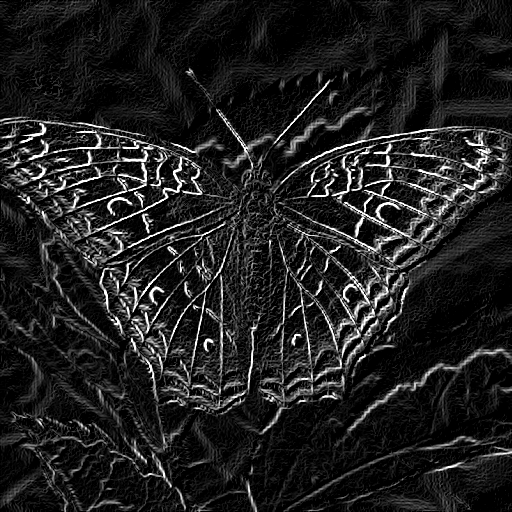
\includegraphics[width=0.9\textwidth]{resultados/butterfly_h3h4.png}
        \caption{Convolução com $h_3$ e $h_4$.}
        \label{fig:sobel:abs}
    \end{subfigure}\\[8pt]
    \begin{subfigure}{0.48\textwidth}
        \centering
        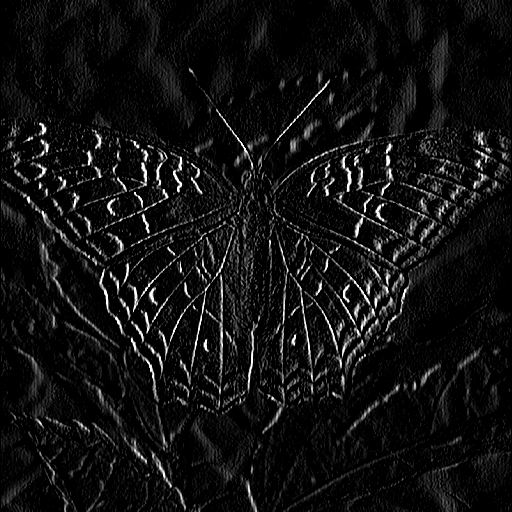
\includegraphics[width=0.9\textwidth]{resultados/butterfly_h3.png}
        \caption{Convolução com $h_3$.}
        \label{fig:sobel:x}
    \end{subfigure}%
    \begin{subfigure}{0.48\textwidth}
        \centering
        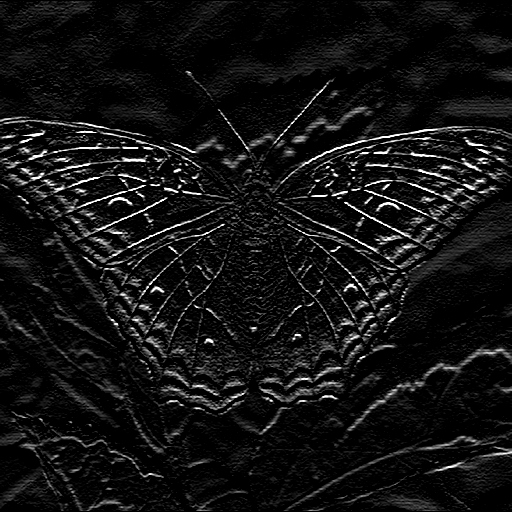
\includegraphics[width=0.9\textwidth]{resultados/butterfly_h4.png}
        \caption{Convolução com $h_4$.}
        \label{fig:sobel:y}
    \end{subfigure}

    \caption{Aplicação dos operadores de Sobel.}
    \label{fig:sobel}
\end{figure}

A aplicação do operador de Sobel, na forma mais completa, pode ser feita no programa por:

\begin{minted}{bash}
    $ python3 main.py imagens/butterfly.png h3 h4
\end{minted}


\subsection{Operador de Prewitt (\texttt{h11})} \label{sec:grad}

    Além do operador de Sobel, existem vários outros operadores baseados em gradiente. Um deles é o de Prewitt \autocite{ref:prewitt}, caracterizado por dois \textit{kernels} $3 \times 3$, com apenas $0$, $1$ e $-1$. No caso da \cref{fig:h11}, o gradiente está apontando para a direção $(-1, -1)$, isto é, da direita-inferior para a esquerda-superior.

Na \cref{fig:grad}, podemos ver claramente o direcionamento pelas antenas da borboleta. A antena esquerda, que está alinhada com o filtro, fica quase indetectada pelo filtro, enquanto a antena direita aparece de forma bem marcada. Além disso, na antena direta, apenas uma das bordas fica marcada, isso porque o filtro não depende apenas da angulação, mas do direcionamento positivo ou negativo naquele ângulo.

O operador de Prewitt, quando usado com direções ortogonais, também pode ser combinado como o de Sobel (\cref{sec:sobel}).

\begin{figure}[H]
    \centering
    \begin{subfigure}{0.48\textwidth}
        \centering
        \begin{kmatrix}
    \matrix[square matrix]{
        -1 & -1 & 0 \\
        -1 & 0 & 1 \\
        0 & 1 & 1 \\
    };
\end{kmatrix}

        \caption{Máscara $h_{11}$.}
        \label{fig:h11}
    \end{subfigure}%
    \begin{subfigure}{0.48\textwidth}
        \centering
        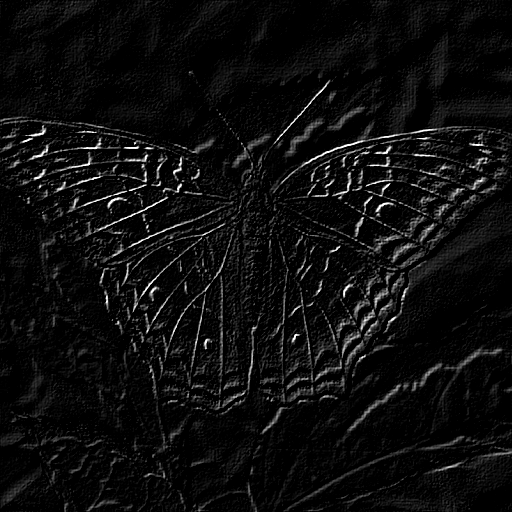
\includegraphics[width=0.9\textwidth]{resultados/butterfly_h11.png}
        \caption{Convolução com $h_{11}$.}
        \label{fig:grad}
    \end{subfigure}

    \caption{Operador de Prewitt, com exemplo.}
\end{figure}

A aplicação do filtro pode ser feita por:

\begin{minted}{bash}
    $ python3 main.py imagens/butterfly h11
\end{minted}


\subsection{Detecção de Linha (\texttt{h7} e \texttt{h8})} \label{sec:linha}

    % https://www.di.univr.it/documenti/OccorrenzaIns/matdid/matdid666794.pdf
% http://www.dpi.inpe.br/spring/teoria/filtrage/filtragem.htm

\begin{figure}[H]
    \centering
    \begin{subfigure}{0.4\textwidth}
        \centering
        \begin{kmatrix}
    \matrix[square matrix]{
        -1 & -1 & 2 \\
        -1 & 2 & -1 \\
        2 & -1 & -1 \\
    };
\end{kmatrix}
        \caption{~$h_1$}
        \label{fig:h7}
    \end{subfigure}%
    \begin{subfigure}{0.4\textwidth}
        \centering
        \begin{kmatrix}
    \matrix[square matrix]{
        2 & -1 & -1 \\
        -1 & 2 & -1 \\
        -1 & -1 & 2 \\
    };
\end{kmatrix}
        \caption{~$h_5$}
        \label{fig:h8}
    \end{subfigure}

    \caption{??}
\end{figure}

\begin{figure}[H]
    \centering
    \begin{subfigure}{0.48\textwidth}
        \centering
        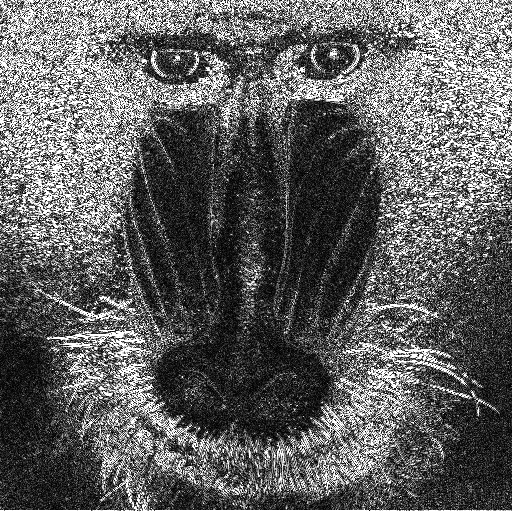
\includegraphics[width=0.9\textwidth]{imagens/baboon.png}
        \caption{Original: \texttt{baboon.png}.}
    \end{subfigure}\\[8pt]
    \begin{subfigure}{0.48\textwidth}
        \centering
        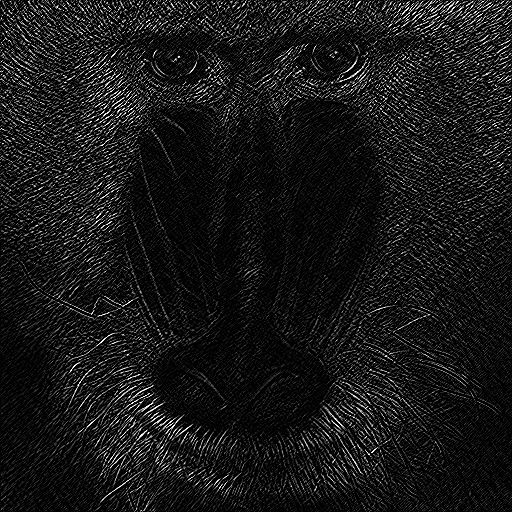
\includegraphics[width=0.9\textwidth]{resultados/baboon_h7.png}
        \caption{Convolução com ??.}
    \end{subfigure}%
    \begin{subfigure}{0.48\textwidth}
        \centering
        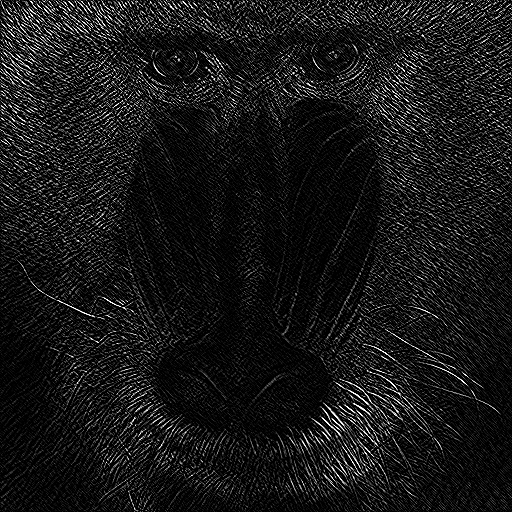
\includegraphics[width=0.9\textwidth]{resultados/baboon_h8.png}
        \caption{Convolução com ??.}
    \end{subfigure}

    \caption{??}
\end{figure}


\subsection{Nitidez (\texttt{h10})} \label{sec:sharpen}

    O último filtro deste trabalho é o de nitidez, também chamado de \textit{sharpen} ou agudização. No espaço das frequências, esse tipo de filtro é responsável por enfraquecer frequências mais baixas, por isso é chamado de filtro passa-altas. Isso faz com que esse filtro seja um tipo processo "inverso" do filtro de \textit{blur} (\cref{sec:blur}).

Assim como os filtros de \textit{blur}, filtros de nitidez têm a soma de seus elementos igual a 1. Isso faz com que o aspecto geral das intensidades da imagem seja mantido. Outra característica interessante desses filtros, é que eles são basicamente uma soma do resultado de um filtro de detecção de borda não direcional com a imagem original. Podemos ver isso comparando as figuras \ref{fig:sharpen:edge}, que é a aplicação do laplaciano em \texttt{city.png}, e \ref{fig:sharpen:sub}, a subtração de \cref{fig:sharpen:sharpen} por \ref{fig:sharpen:orig}.

\begin{figure}[H]
    \centering
    \begin{kmatrix}
    \matrix(img)[square matrix]{
        -1 & -1 & -1 & -1 & -1 \\
        -1 & 2 & 2 & 2 & -1 \\
        -1 & 2 & 8 & 2 & -1 \\
        -1 & 2 & 2 & 2 & -1 \\
        -1 & -1 & -1 & -1 & -1 \\
    };

    \node[left=of img] {$\displaystyle\Scale[1.7]{\frac{1}{8}}$};
\end{kmatrix}

    \caption{Máscara de nitidez: $h_{10}$.}
    \label{fig:h10}
\end{figure}

\begin{figure}[H]
    \centering
    \begin{subfigure}{0.48\textwidth}
        \centering
        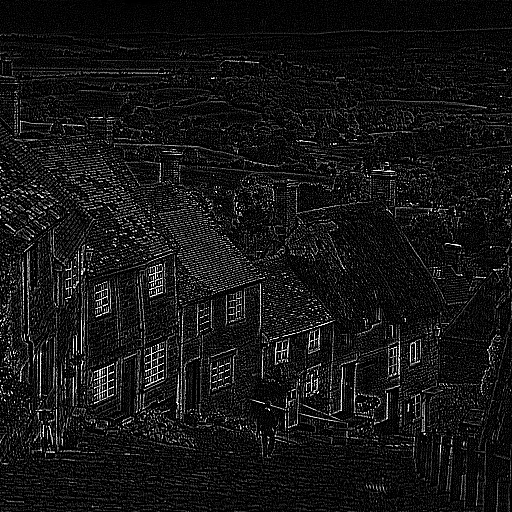
\includegraphics[width=0.9\textwidth]{imagens/city.png}
        \caption{Original: \texttt{city.png}.}
        \label{fig:sharpen:orig}
    \end{subfigure}%
    \begin{subfigure}{0.48\textwidth}
        \centering
        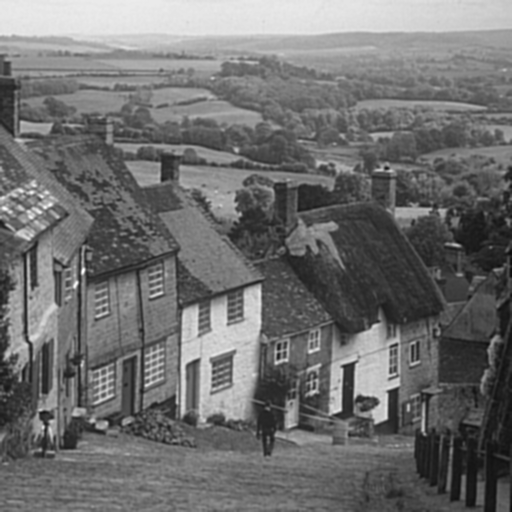
\includegraphics[width=0.9\textwidth]{resultados/city_h2h10.png}
        \caption{Convolução com $h_2$, depois com $h_{10}$.}
        \label{fig:sharpen:combinada}
    \end{subfigure}\\[8pt]
    \begin{subfigure}{0.48\textwidth}
        \centering
        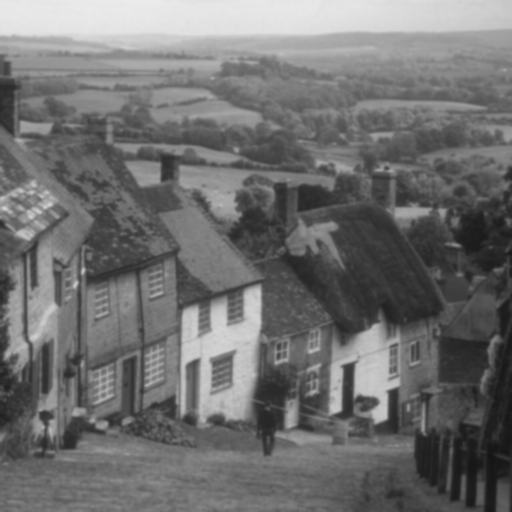
\includegraphics[width=0.9\textwidth]{resultados/city_h2.png}
        \caption{Convolução com $h_2$ (\ref{fig:h2}).}
        \label{fig:sharpen:blur}
    \end{subfigure}%
    \begin{subfigure}{0.48\textwidth}
        \centering
        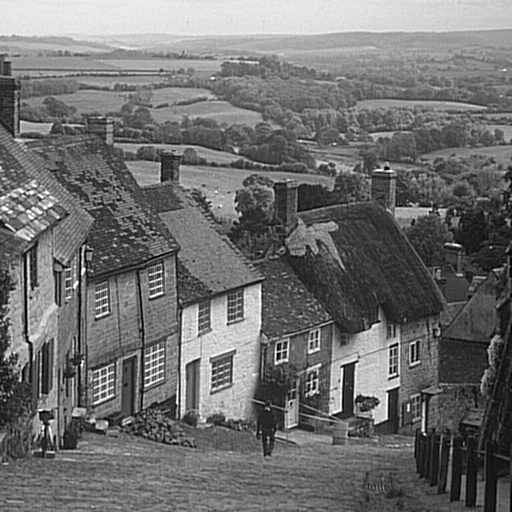
\includegraphics[width=0.9\textwidth]{resultados/city_h10.png}
        \caption{Convolução com $h_{10}$ (\ref{fig:h10}).}
        \label{fig:sharpen:sharpen}
    \end{subfigure}\\[8pt]
    \begin{subfigure}{0.48\textwidth}
        \centering
        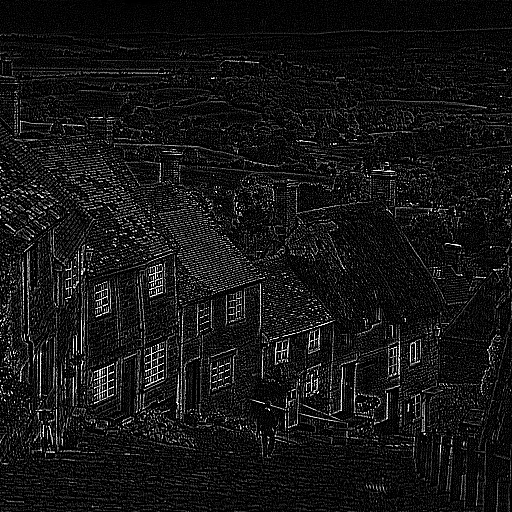
\includegraphics[width=0.9\textwidth]{resultados/city_h5.png}
        \caption{Convolução com $h_5$ (\ref{fig:h5}).}
        \label{fig:sharpen:edge}
    \end{subfigure}%
    \begin{subfigure}{0.48\textwidth}
        \centering
        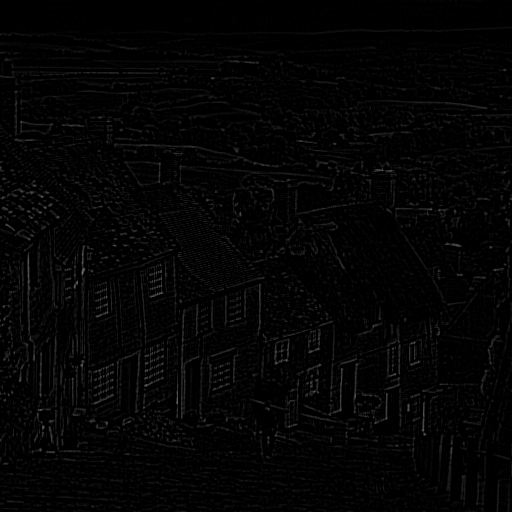
\includegraphics[width=0.9\textwidth]{resultados/city_h10e.png}
        \caption{Convolução com $h_{10}$, removido da original.}
        \label{fig:sharpen:sub}
    \end{subfigure}

    \caption{Filtros de \textit{blur} e de nitidez.}
\end{figure}

Podemos ver nas figuras \ref{fig:sharpen:blur} e \ref{fig:sharpen:sharpen}, comparando com a original (\ref{fig:sharpen:orig}), que o \textit{blur} ($h_2$) reduz a nitidez, enquanto o \textit{sharpen} ($h_{10}$) aumenta. Aplicando o filtro $h_2$ e o $h_{10}$, nessa ordem, resulta na \cref{fig:sharpen:combinada}, que tem nitidez comparável com a original.

A execução desse filtro é pode ser feita com:

\begin{minted}{bash}
    $ python3 main.py imagens/city.png h10
\end{minted}


\subsection{Argumentos Opcionais}

    Na \cref{fig:opt} podemos ver o resultado da mesma operação da \cref{fig:borda:viz4}, que é o \hyperref[fig:h1]{filtro $h_1$} da \cref{sec:borda}, mas com os argumentos opcionais \mintinline{bash}{-t} (\cref{sec:impl:t}) e \mintinline{bash}{-n} (\cref{sec:impl:n}). Os resultados acabaram ficando mais difíceis de analisar, por isso as opções padrões foram utilizadas em todo o projeto.

    \begin{figure}[H]
        \centering
        \begin{subfigure}{0.48\textwidth}
            \centering
            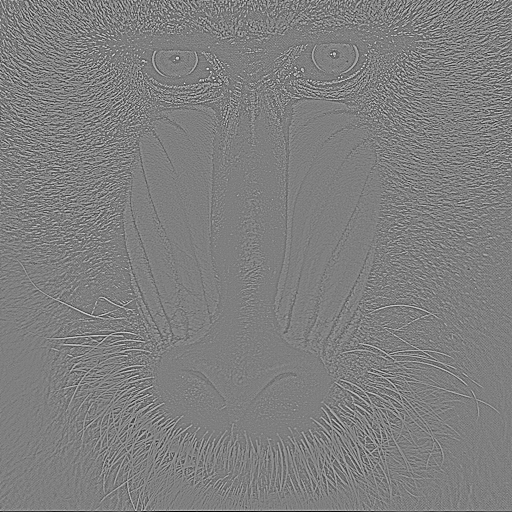
\includegraphics[width=0.9\textwidth]{resultados/baboon_h1t.png}
            \caption{Argumento \mintinline{bash}{-t}.}
            \label{fig:opt:t}
        \end{subfigure}%
        \begin{subfigure}{0.48\textwidth}
            \centering
            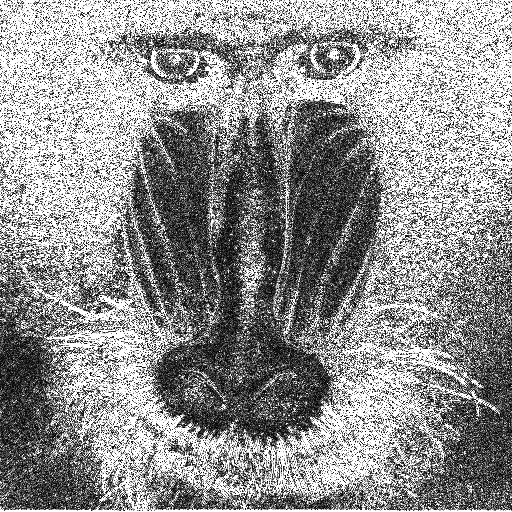
\includegraphics[width=0.9\textwidth]{resultados/baboon_h1n.png}
            \caption{Argumento \mintinline{bash}{-n}.}
            \label{fig:opt:n}
        \end{subfigure}

        \caption{Resultados com os argumentos opcionais.}
        \label{fig:opt}
    \end{figure}

